
\section{Context-free grammars}


Now that we have seen a grammar given by production rules we can explain 
in what way context-free grammars are ``context-free'', and how they 
come to parse as trees.  Consider the situation discussing square-roots 
of natural numbers.
\begin{center}
\begin{gcode}[]
+<Root> ::= + sqrt(<Nat>)
-<Root> ::= - sqrt(<Nat>)
\end{gcode}
\end{center}
In this case \code{sqrt{2}:<Root>}.  However, we do not know if this 
was meant as the positive or negative root.  That information 
was left to the surrounding context in which the term was parsed.  
This is a very useful situation as often in algebra we do want to 
speak within a context.  Yet because of the ambiguity if we 
introduce a root in this way and then seek to eliminate we 
cannot be certain of many possible paths got us here.

Meanwhile 
to make this context-free grammar we could use 
\begin{center}
\begin{gcode}[]
<Root> ::= + sqrt(<Nat>)
         | - sqrt(<Nat>)
\end{gcode}
\end{center}
Now \code{+sqrt(2):<Root>} and \code{-sqrt(2):<Root>} but 
this grammar rejects \code{sqrt(2)}.  The grammar is less forgiving 
but more precise in the content it now holds for us.

\begin{definition}
    A \emph{context-free grammar} is a grammar whose non-constant 
    production rules are defined on their to the left of the astonished Walrus 
    \code{::=}.
\end{definition}

For example, productions rules that begin in the form \code{<Thing>::=...}
are all that we permit.

\begin{definition}
    The \emph{parse-graph} of an accepted string $\sigma$ is 
    defined recursively as the having vertices any production rule 
    which ends in a terminal equal ot $\sigma$, or 
    if $\sigma$ is non-terminal, then vertex for each production rule 
    that accepts $\sigma$ with an edge to any production rules traversed
    by that acceptance.
\end{definition}

\begin{proposition}
    The parse graph of an accepted string of an unambigiuous context free grammar 
    is a unique vertex-labeled tree, with each label a production rule and each leaf 
    an atom (constant/variable symbol).
\end{proposition}
\begin{proof}
    Suppose $x$ is accepted as $x:Token$.  
    Because the grammar is an unambigious grammar 
    it has a unique token that accepts $x$.
    As it is context-free we are guaranteed 
    that $x$ was accepted by a production rule of form 
    \code{<Token>::= A1 ... An} where the 
    \code{Ai}'s are 
    terminal or production rules.  By recursion assign 
    to each \code{Ai} its associated parse graph which
     by induction makes each into a rooted tree.
\end{proof}

A further property that we often exploit but we shall not prove here is that 
context-free grammars are economical to parse.  In fact they do not even 
require the full strength of a computer but could be done with the type 
of system needed to program a microwave.  While Moore's law drove the creation 
of full strength (Turing Complete) microprocessors, the need to reduce energy 
and cost of production has brought a resurgence of such limited ability 
hardware.  
\begin{proposition}
    A context free grammar can be parsed by an automata with a push-down (last-in-first-out)
    stack.
\end{proposition}

For comparison, to parse context-sensitive grammars we suddenly require more 
than Turing machine, we need a nondeterminisitc machine.  That is, we have to make 
some (possibly random) choices about what way to parse.

\subsection{$\mathbb{N}$ as an algebra}
Although we have come to know $\mathbb{N}$ for its addition take note that 
the real work was done by the successor.  In fact the introductions themselves 
point the way to the founding operations of natural numbers.
\begin{enumerate}
    \item The $0$ operator converts nothing into a starting point.  
    \item The successor operator \code{S<Nat>}, abbreviated now to just 
    $S\Box$, converts a given natural number into a new one.
\end{enumerate}

Addition is different from $S$ because addition is not making new 
numbers, it is actually just refashioning numbers into others.  


\begin{remark}
    Many argue that natural numbers should not contain $0$ because we start counting 
    at $1$.  Others argue that because of natural numbers have a place to start 
    and call it what you like the starting place always behave like $0$ when we add.

    Both perspectives have a point but both traffic in a misrepresentation of the 
    situation.  To say that there is a place to start, call it 0, is to say 
    you can begin a tally.  But the act of counting is to tally, that is, the case 
    of $+$, resp. \code{S}. So from $0$ our first count is $1\defeq S(0)$. 
    
    So it transpires that the
    natural numbers do include $0$ (an empty tally board), but at the same time
    we begin counting at $1$.  Neither point of view is possible without the other
    being true.
\end{remark}

In mathematics two paths to the same place are said to be a relation.  So systems that have no cycles, i.e.\ trees, are 
free of relations, or simply \emph{free}.  In time we will come to see 
that every algebraic structure can be constructed from a free 
structure with the possible addition of relations.

\begin{remark}
    Having two formulas that reduce to the same value is not the same 
as a relation in the grammar.  So what is free in this case 
is the grammar we used for arithmetic formulas.  
For example $7(7+3)(7+3)$ renders the same result 700, and nearly 
by the same steps.  Yet, if we diagrammed that formula as a
parse tree it would quite different
\begin{center}
    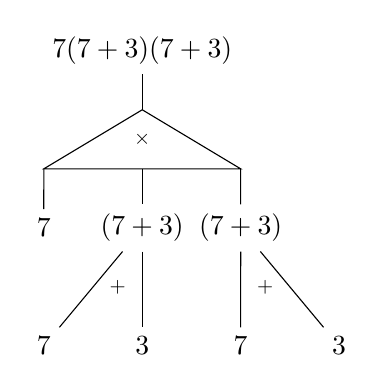
\begin{tikzpicture}[xscale=1.25,yscale=0.75]
        \node (t) at (0,1) {$7(7+3)(7+3)$};
        \node (a) at (-1,-2) {$7$};
        \node (b) at (0,-2) {$(7+3)$}; 
        \node (c) at (1,-2) {$(7+3)$};
        \node (e) at (-1,-4) {$7$};
        \node (f) at ( 0,-4) {$3$};
        \node (g) at ( 1,-4) {$7$};
        \node (h) at ( 2,-4) {$3$};

        \draw (0,0) -- (-1,-1) -- (1,-1) -- cycle;

        \node[scale=0.75] at (0,-0.5) {$\times$};
        \node[scale=0.75] at (-0.25,-3) {$+$};
        \node[scale=0.75] at ( 1.25,-3) {$+$};

        \draw[-] (t) -- (0,0);
        \draw[-] (-1,-1) -- (a);
        \draw[-] (0,-1) -- (b);
        \draw[-] (1,-1) -- (c);
        \draw[-] (b) -- (e);
        \draw[-] (b) -- (f);
        \draw[-] (c) -- (g);
        \draw[-] (c) -- (h);
    \end{tikzpicture}    
\end{center}    
In particular we have not even expressed this as a pair of products 
we have asked instead for a function that takes products of three 
numbers at once.  The ambiguity of how we might achieve this is hidden in the 
triangle \emph{operad} labeled $\times$.
\end{remark}

\subsection{Formal definitions}

